\documentclass{style/llncs}

\usepackage{amsmath,amsfonts}
\usepackage{color}
\usepackage[usenames,dvipsnames,svgnames,table]{xcolor}
\usepackage[mathscr]{eucal}
\usepackage{thmtools}
\usepackage{graphicx}
\usepackage{caption}

\newcommand{\M}{\mathscr M}
\newcommand{\C}{\mathscr C}
\newcommand{\T}{\mathscr T}
\newcommand{\F}{\mathscr F}
\renewcommand{\P}{\mathscr P}
\newcommand{\K}{\mathscr K}
\newcommand{\X}{\mathscr X}
\newcommand{\B}{\mathbb B}
\newcommand{\D}{\Delta}
\newcommand{\N}{\mathbb N}
\newcommand{\tn}[1]{\textnormal{#1}}
\newcommand{\pair}[1]{\left\langle{#1}\right\rangle}
\newcommand{\concat}{\oplus}
\newcommand{\symb}[1]{\texttt{#1}}
\newcommand{\br}[1]{\overline{#1}}
\newcommand{\s}{S}
\newcommand{\bi}{\bar\imath}
\newcommand{\dom}[1]{\mathop{\tn{dom}(#1)}}
\newcommand{\range}[1]{\mathop{\tn{range}(#1)}}

\newtheorem{conj}{Conjecture}

\let\doendproof\endproof
\renewcommand\endproof{~\hfill\qed\doendproof}

\newcommand{\p}{\,\text{.}}

\newcommand{\tuple}[1]{\left\langle{#1}\right\rangle}

\newcommand{\hide}[1]{}
\newcommand{\old}[1]{}

\newcommand{\sdr}[1]{\textcolor{blue}{\small #1\textsuperscript{[Steven]} }}
\newcommand{\pb}[1]{\textcolor{OliveGreen}{\small #1 \textsuperscript{[Peter]} }}

\newcommand{\argmin}{\mathop{\arg\min}}


\title{Two Problems for Sophistication}

\author{Peter Bloem and Steven de Rooij}

\institute{
  System and Network Engineering Group, \\University of Amsterdam, the Netherlands\\
  \email{uva@peterbloem.nl, steven.de.rooij@gmail.com}
}

\begin{document} 
\maketitle

\begin{abstract}
Kolmogorov complexity measures the amount of information in data, but does not distinguish structure from noise. Kolmogorov's definition of the \emph{structure function} was the first attempt to measure only the structural information in data, by measuring the complexity of the smallest model allowing for optimal compression of the data. Since then, many variations of this idea have been proposed, for which we use \emph{sophistication} as an umbrella term. We describe two fundamental problems with existing proposals, showing many of them to be unsound. Consequently, we put forward the view that the problem is fundamental: it may be impossible to objectively quantify the sophistication.
\end{abstract}

\section{Introduction}

Kolmogorov complexity gives us a sound definition of the amount of information contained in a binary string. It does not, however, capture what most people would consider complexity. For example, a sequence of a million coin flips will almost certainly have maximal Kolmogorov complexity, even though there is nothing complex about flipping a coin repeatedly. Many scholars have defined additional complexity measures in the spirit of Kolmogorov complexity, aimed at quantifying not \emph{all} information in a binary string, but only the \emph{meaningful} information. While this concept has been given many names, we use \emph{sophistication} as an umbrella term. In this paper, we investigate two serious problems with sophistication measures. We conclude with three arguments that suggest the problems are fundamental, explaining our belief that sophistication cannot be defined in a satisfactory manner.

The Kolmogorov complexity $C(x)$ of a binary string $x$, is (roughly) the length of the shortest computer program that will output $x$. This length depends on which programming language is used, but, as shown by a central result known as the invariance theorem \cite[Section~2.1]{li1993introduction}, the language affects the value only by a constant, independent of $x$. This means that for sufficiently complex objects, the choice of programming language becomes irrelevant and Kolmogorov complexity becomes an \emph{objective} measure of the complexity of binary strings, a property \emph{of the data.} A definition of sophistication $S(x)$ in the spirit of Kolmogorov complexity should have similar robustness guarantees:

\begin{enumerate}
\item $S(x)$ should count the bits required for an effective description of the structural properties of a binary string.
\item An analogue of invariance should hold: there must be strict limits on how much sophistication can be affected by a change in programming language.
\item There should be no constant $c$ such that $S(x)\le c$ for every input $x$. If sophistication is bounded, then knowing its value under one programming language provides no constraints on its value under another language (except that it's also bounded). Moreover, a bounded sophistication would be at odds with the intuition that there is no limit to the amount of structure that a binary string can exhibit.
\item Similarly, there should be no constant $c$ such that $C(x)-S(x)\le c$ for all $x$, because then sophistication would be equivalent to Kolmogorov complexity. 
\end{enumerate}
There have been many related proposals for such a measure, all based on a \emph{two-part code}: rather than encoding $x$ by means of a single computer program, we encode a \emph{model} for $x$ in the first part of the code, which is interpreted as a representation of $x$'s structural properties. The model does not fully specify $x$, but when combined with the second part of the code, which specifies the noise, the original string becomes fully determined. Thus, the model can be interpreted as a function mapping the noise to the original object.

For any string $x$, there may be many different two-part representations. The total codelength can never be less than the Kolmogorov complexity, but it can come close. The balance between the two parts may vary; Figure~\ref{fig:diagram} provides an illustration. The various proposals then define sophistication in terms of the length of the structure part of this two-part code for one of the representations that (almost) achieves the Kolmogorov complexity. However, for most of these definitions, we can prove that they fail one or more of the conditions above. Vit\'anyi's definition \cite{vitanyi2004meaningful} is the one exception that we cannot \emph{prove} to conflict with our requirements, but we show that this method only assigns substantial sophistication to strings that require an enormous amount of processing to construct.

\begin{figure*}[tb]
  \centering
  \begin{minipage}{0.45\textwidth}
     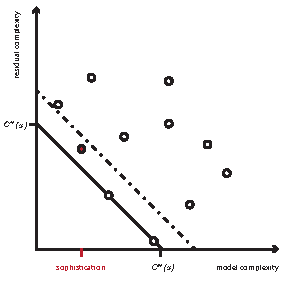
\includegraphics[width=\textwidth]{./img/sophistication.pdf}
  \end{minipage}
  \begin{minipage}{0.45\textwidth}
     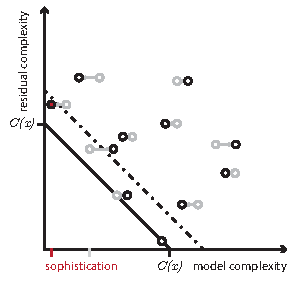
\includegraphics[width=\textwidth]{./img/sophistication-jump.pdf}
  \end{minipage}
  \caption{\small (left) Two-part representations of $x$ by the two components of their codelength. The Kolmogorov complexity $C^\M(x)$, appearing as a black diagonal, provides a lower bound on the total codelength. We consider only representations that are close to this optimum, with the threshold represented by a dashed line. The size of the smallest model below the threshold is the sophistication of the data. (right) The same image, after a constant perturbation in the model complexity caused by a change in numbering.}
  \label{fig:diagram}
\end{figure*}

A valid definition of $S$ must contend with two important issues. First, the details of the way the model is encoded are important. There are two technically distinct approaches; in one of these one has to deal with the so-called ``nickname problem'' that strangely remains unresolved in several publications. These definitions yield a sophistication that is highly dependent on the chosen programming language, unless special care is taken, as discussed in Section~\ref{section:indices}.

The second issue is that of striking the right balance between underfitting and overfitting, which we consider in Section~\ref{section:balance}. Overfitting is a common problem in the statistical literature, that refers to the tendency of model selection to choose a complex model that provides a very good fit to the observed data, but does not generalise well to unseen data. In the case of sophistication, overfitting occurs if the model that determines the sophistication contains much or even all of the noise. This is a real danger, because the models are encoded so efficiently. In statistics, overfitting is often addressed by penalising complex models. In sophistication, however, such penalties tend to break the balance between structural information and noise, and lead to the opposite problem: underfitting.

Underfitting occurs when the selected model is simple, but fails to represent some of the structure present in the data. This is also a problem for sophistication because the models under consideration are so powerful. In particular, in any programming language, there are programs that implement an interpreter for \emph{another} language. Such \emph{universal models} are \emph{simple} in the language of sophistication, since they can be described with a relatively small number of bits, yet are able to represent the data within a codelength a constant away from the Kolmogorov complexity. Such a two-part representation essentially encodes all information as noise. If complex models are penalized, then the problem becomes to make sure that universal models are not \emph{always} preferred for complex data. The usual workaround is to restrict the set of allowed models to exclude the universal ones. For example, the model class may be restricted to the set of all total recursive functions. While this excludes universal models, it is questionable whether it adequately solves the problem of underfitting in general.

Finally, in the discussion in Section~\ref{section:conclusion} we argue that while two-part coding can yield useful insights into the structure of the data and allows us to identify some models as poor representations, it is probably not possible to uniquely separate structure from noise and identify a \emph{single} model as ``best'': in general many models, of vastly different complexities, may be reasonable representations. Rather than doggedly trying to ``fix'' this property of algorithmic statistics, we propose embracing the idea that the data allows for multiple equivalent interpretations of which information is structured, and which is random, and that there is no such thing as sophistication.

\section{Preliminaries}
One of the main issues in dealing with sophistication in a general sense, is that one must unify many different approaches, all founded on slightly different principles. We have devised a general framework which, while it may not represent the idiosyncracies of all methods, allows us to rephrase them in a uniform way that illustrates the properties we discuss. We hope the reader will trust that these properties remain also in the original statements of the measures.

Let $\B = \{0,1\}^*$. We deal with partial computable functions $f: \B \times \B \to \B$, which we will also call \emph{models}. A function is called \emph{prefix} if its domain, $\dom{f} = \{y : f(y; \cdot) \neq \infty\}$ is a prefix free set, i.e. no string in $\dom{f}$ is a prefix of another. A function $f$ is \emph{total} if $\dom{f} = \B$. In most cases, we do not use the second argument, and we adopt the convention that $f(x) = f(x, \epsilon)$.

A \emph{numbering} is an enumeration of of the partial computable functions, denoted as $\psi_1, \psi_2, \ldots$ or simply $\psi$. We fix one canonical effective numbering $\phi$. We call a numbering $\psi$ \emph{acceptable} if there exist total, computable functions $a, b: \N \to \N$ with $\forall: i$, $\phi_i = \psi_{b(i)}$ and  $\psi_i = \phi_{a(i)}$.

A \emph{model class} is a set of model indices. We distinguish four important model classes:
\begin{itemize} 
  \item The indices of the partial computable functions $\C=\N$.
  \item The total functions $\T=\{i:\tn{$\phi_i$ is total}\}$. Note that $\T$ is not computably enumerable.
  \item $\K$ is an enumerable set such that $\{\phi_i:i\in\K\}$ is the set of all partial computable prefix functions.
  \item The finite sets: $\F$ is an enumerable set such that $\{\phi_i:i\in\F\}$ contains a uniform code for every finite set. A uniform code for a finite set $S$ is a total computable surjective function $f:\{0,1\}^{\lceil\log|S|\rceil}\to S$.
\end{itemize}

We sometimes need to map binary strings to a prefix-free set. We denote by $\br{x}$ the prefix-encoded representation for $x$. We require that the mapping satisfies $|\br{x}| = |x|+O(\log(|x|)$ (see eg. \cite[Section~1.4]{li1993introduction}). To simplify notation, we will sometimes conflate natural numbers and binary strings, implicitly using the ordering $(0, \epsilon)$, $(1, 0)$, $(2, 1)$, $(3, 00)$, $(4, 01)$, \ldots  

For technical reasons, we deviate slightly from the traditional notation of Kolmogorov complexity: we define the $\M$-Kolmogorov complexity of a binary string $x$, with respect to a model class $\M$ and a numbering $\psi$, as follows $C^{\M,\psi}(x\mid z)=\min\{\bar\imath y:\psi_i(y; z)=x,i\in\M\}$, with $C^\M(x) = C^\M(x\mid \epsilon)$. This means that $C^\C(x)$ corresponds to the plain Kolmogorov complexity, traditionally denoted $C(x)$, and $C^\K(x)$ corresponds to the prefix-free Kolmogorov complexity $K$. This notation also allows us to represent the smallest possible description of $x$ using a single model $\phi_i$ as $C^{\{i\}}(x)$. Note that this includes the description of $i$ as well as its shortest program for $x$.

Finally we note that the choice of numbering, combined with a choice of prefix function, serves the same purpose that is normally expressed in the choice of a Turing machine. Requiring an acceptable numbering and a computable prefix function is equivalent to choosing a universal Turing machine: this requirement suffices to make the Kolmogorov complexity invariant. As we shall see, however, this is not enough for a proper treatment of sophistication: we must choose our numbering with care. Thus, we phrase our requirement for an invariant sophistication with respect to the \emph{numbering} chosen. There should be strict guarantees on how much the value of $S(x)$ can change if the numbering is varied.
 
\section{Inefficient indices}
\label{section:indices}

The simplest approach to sophistication would simply be to `open up' the Kolmogorov complexity and to see which program on the universal Turing machine achieves the smallest description length: the program that \emph{witnesses} the Kolmogorov complexity. Since any UTM is defined in terms of a two-part coding, such programs necessarily consist of a model and an input. As is common, we will allow all witnesses within a constant slack term $c$ from the Kolmogorov complexity, and choose the one with the smallest model.

\begin{definition}[Index sophistication]
\[
\s_{\text{index}}^{\M_1,\M_2,\psi,c}(X) = \min\left\{ |i| : \i \in \M_1, C^{\{i\}, \psi}(x) \leq C^{\M_2, \psi}(x)+c   \right\}
\]
When $\M_1 = \M_2$, we will abbreviate with $\s^{\M_1,\psi,c}$
\end{definition}

Koppel and Atlan's treatment \cite{koppelSoph1988,koppel1991almost}, where the name \emph{sophistication} originates, follows this basic logic, although it contains many idiosyncracies like the use of monotonic models, and an inherent extension to infinite strings. As the subsequent history of sophistication has discarded these, we will not discuss them here.

In \cite{antunes2009sophistication,antunes2013sophistication} Koppel's principle is recast to finite strings. The definition used is similar to $s_\text{index}^{\T, \C,\psi,c}$, with one exception: the total complexity of a witness $(i,y)$ is measured as $|i|+|y|$ without the cost of delimiting the two. This difference is not relevant to the point we make in this section. The restriction to total classes is a common technique to avoid underfitting, which we will discuss in the next section. 

\begin{lemma}
Let $s^\psi$ denote any index sophistication with respect to numbering $\psi$.
There are acceptable numberings $\psi$ and $\xi$ such that for all $x$:\\
\-\hspace{2.8em} $|s^\psi(x) - s^\xi(x)|\geq \tfrac{1}{2}\min\{s^\psi(x),s^\xi(x)\}$.
\end{lemma}
\begin{proof}
Let $s_i$ be the string consisting of $2^{i}$ zeroes followed by a one. Define $\phi, \xi$ such that $\psi_j(x) = \phi_i(x)$ for $j = s_{2i}$ and $\xi_j(x) = \phi_i(x)$ for $j = s_{2i+1}$, with all other functions returning $\infty$. Choose any $x$ and assume w.l.o.g. that $s^\psi(x)\le s^\xi(x)$. By construction, we have $2s_\psi(x)  \leq s_\xi(x)$ from which the lemma follows.
\end{proof}
Thus, the length of the index is a very poor indicator of model complexity. In order to obtain a robust measure, define the complexity of functions as in \cite{grunwald2004shannon,vitanyi2004meaningful} by $C^{\M,\psi}(f) = \min\{C^{\M,\psi}(i):\phi_i=f\}$.
Lemma~\ref{lemma:invariance} in the appendix shows that this definition is invariant: it is an objective property of a function.

Note that such perversely inefficient numberings are not an issue for Kolmogorov complexity. If our universal Turing machine uses an inefficient numbering, we can switch to a more efficient one at only a constant cost. This gives us an insight into what happens inside Kolmogorov complexity. We may define the program $\bi y$ using a model $i$ and an input $y$, but if there's any inefficiency in the description of $i$, the shortest program will be achieved by using $i$ to define a more efficient model encoding, and encoding both the model and its input in $y$. For the Kolmogorov complexity, such considerations are academic, since we only look at the total length of the program. For sophistication, however, they are crucial.

There are two ways to use the model complexity $C^\M(\phi_i)$ for more robust attempts to define sophistication. Confusingly, both are used in the literature. First, we can measure the complexity of the \emph{model} using $C^{\M,\psi}(\phi_i)$, which is then the first part of a two-part code describing the data. This approach is used in  \cite{cover1985kolmogorov,gacs2001algorithmic,vitanyi2004meaningful,gellmann1996information} and in most of the present paper.

Second, we can stick to using the length of the index as the measure of sophistication, but restrict the allowed numberings. This approach is taken is in \cite{adriaans2012facticity}. Adriaans  defines \emph{facticity} as $\s_\text{index}^{\C,\psi,0}$, but only allows numberings that are \emph{faithful}: for all $i$ there is a $j$ such that $\psi_i=\psi_j$ and $|j|\le C^{\C}(\psi_j)+c$, for some constant $c$.

We prove in the appendix that---contrary to Adriaans' suggestion---there actually do exist faithful, acceptable numberings (Lemma~\ref{lemma:faithful-numberings}). However even choosing a faithful index is not quite enough. The Kolmogorov complexity uses representations of the form $\bar\imath y$, where the bar denotes some straightforward prefix encoding to delimit the model description $i$ from its input $y$. If we define a second prefix encoding $\tilde{\imath}$, with $|\bar\imath|-|\tilde\imath|$ unbounded, we can define a second representation $\bar u \tilde \imath y$, at a constant overhead $|\br{u}|$, and gain more than $|\br{u}|$ for sufficiently complex strings. As shown in Lemma~\ref{lemma:prefix-inefficiency} in the appendix, this results in a bounded sophistication (thus the facticity is bounded). 

Because of these issues, rather than index sophistication we will use the following definition of sophistication in the remainder of this article. It is parameterised by a model class, a numbering, and a slack parameter $c$ that determines the maximal allowed slack between the two-part code length using a representation and the Kolmogorov complexity.
\[
\s^{\M_1,\M_2,\psi,c}(x)=\min\left\{C^\K(\phi_i):i\in\M_1,C^{\{i\},\psi}(x)\le C^{\M_2,\psi}(x)+c\right\}.
\]

\section{Balancing under- and overfitting}
\label{section:balance}

In the previous section, we saw the first glimpse of the delicate balance between the two code components in sophistication. We will investigate this balance, starting with the variant $\s^{\K,\psi,c}$. For reasons which will become clear, this variant is not used anywhere in the literature, but it helps to illustrate the issues we wish to discuss.

In this setting, we know that, on the one hand, there always exist witnesses for which all information except a constant amount is stored in the input, and on the other hand, there are also candidate representations for which all information is stored in the model. This tells us that $S^\K$ is \emph{balanced}: there is no inefficiency in the representation forcing information in or out of the model.
The flip side of having a balanced sophistication is that it becomes easy to show a lack of invariance, by tweaking the numbering in such a way that models in a specific subset $\M'\subset\M$ of the model class becomes an arbitrary constant number of bits cheaper to represent than all other models, so that a model in $\M'$ always ends up determining the sophistication.

This means that for model classes with a universal model, we can choose our numbering to make $S^\K$ bounded, or equal to the complexity:

\begin{restatable}[Underfitting]{lemma}{underfitting}
Let $\M$ be a model class containing a universal model $\phi_u$, with the property that $\exists c \forall i \in \M : C^{\{u\}}(x) \leq C^{\{i\}}(x) + c \p$. Then, there exist numberings such that $\s^\M$ is bounded.\label{lemma:underfitting}
\end{restatable}

For this reason, many treatments restrict the model class. What is perhaps less well known is that the same property holds in the other direction: there are numberings for which the singleton models always determine the sophistication. 

\begin{restatable}[Overfitting]{lemma}{overfitting}
Let $\M \subseteq \K$ be a model class where for every $x\in\X$ there is a singleton model $i\in\M$ with $\phi_i(\epsilon)=x$. Then there is a numbering $\psi$, and a constant $c$, such that for all $x\in\X$ we have $C^\M(x)-S^{\M,\psi}(x)\leq c$.\label{lemma:overfitting}
\end{restatable}

The proof of both these lemmas relies on a simple principle: for certain subclasses $\M' \subset \M$, there exist numberings which, when used, have the effect of penalizing the codelength $C^\K(\phi_i)$ for any model outside $\M'$ by an arbitrary constant amount. We can use this penalty to effectively `push' these models outside of the range of considered models, ensuring that, under this numbering, a model in $\M'$ always determines the sophistication.

For the lemmas above, this means setting $\M' = {u}$, with $\phi_u$ a universal model, or letting $\M'$ be the set of all singletons. The requirements for $\M'$ are strict, and slightly complex. The following lemma gives a set of sufficient conditions.

\begin{restatable}{lemma}{coolone}
\label{lemma:thecoolone}
  Let $\M$ be any model class, let $\X$ be any set of binary strings and let $D:\B\to\N$ be a computable decoding function with a prefix-free domain that maps function descriptions to their indices in $\phi$, i.e. if $m=\phi_{D(p)}$ then $p$ is a $D$-description of $m$. Let $\M'=\{\phi_i:i\in\tn{range}(D)\}$. Further assume there is a constant $c$ such that:\\
\-\hspace{1cm}(1) $\forall_{m\in\M'}:\min\{|p|:\phi_{D(p)}=m\}\le C^{\K,\phi}(m)+c$\\
\-\hspace{1cm}(2) $\forall_{x\in\X}:C^{\M',\phi}(x)-C^{\M,\phi}(x)\le c$.\\
Then there is an enumeration $\psi$ of the partial recursive functions such that $S^{\M,\psi}(x) = |\br{0}|+S^{\M',\phi}(x)$ for all $x\in\X$.
\end{restatable}

\begin{proof}
We define the numbering $\psi$ as follows:
\[\begin{cases}
\psi_0(p) = 1^r 0 D(p) \\
\psi_{1^r0i}(p) = \phi_i(p) \\
\psi_j(\cdot) = \infty &\text{if $j$ contains no zeroes.}
\end{cases}\]
We will show that under the $\psi$-enumeration, the best representation for $x$ using a model $m\in\M'$ is always better than the best representation using some $m\notin\M'$.

First suppose $m\in\M'$. Then
\begin{align*}
C^{\K,\psi}(m) &=\min\{|\bar\jmath q|:\psi_{\psi_j(q)}=m\}
\leq\min\{|\bar0 q|:\psi_{\psi_0(q)}=m\} \\ 
&=\min\{|\bar0 q|:\psi_{1^r0 D(q)}=m\}  
=\min\{|q|:\phi_{D(q)}=m\} + |\bar 0|\\
&\leq C^{\K,\phi}(m)+c+|\br{0}|,
\end{align*}
where the last inequality uses assumption (1).

Now assume that the best model $m$ for $x$ is not in $\M'$. 
Let $i$ be the index of $m$ with the shortest description, i.e. it achieves the minimum in $C^{\K, \psi}(m)=\min\left\{C^{\K,\psi}(i):\psi_i=m\right\}$.
There are two possibilities. Either $i = 0$, in which case we have $C^{\K,\psi}(m)\ge r$ because $\phi_0$ cannot output zero and all other $\psi$-programs are at least $r$ bits long.

Otherwise, we can bound
\begin{align*}
C^{\K,\psi}(m)&=C^{\K,\psi}(i)=C^{\K,\psi}(1^r0j)\\
&\ge C^{\K,\psi}(j)-c' \ge C^{\K,\phi}(j)+r+1-c'\\
&=C^{\K,\phi}(m)+r+1-c'.
\end{align*}
Now choose $r=c''+\max\left\{C^{\K,\psi}(\phi_0),c'-1\right\}$. Then substitution yields, for both cases, 
$C^{\K,\phi}(m)\ge c''+C^{\K,\psi}(m)$.

Combining the inequalities above, for any model $g\not\in\M'$, there is a model $f\in\M$ such that
\[\begin{split}
C^{\K,\psi}(g)+\min \{|y| : g(y) = x\} &\ge C^{\K,^\phi}(g)+\min\{|y| : g(y) = x\}+c''\\
&\ge C^{\K,\psi}(f)+\min \{|y| : f(y) = x\} -2c+c'' -|\bar0|.
\end{split}\]
By choosing $c''$ sufficiently large, we can ensure that the best representation is in $\M'$ for all $x\in\X$, which completes the proof.
\end{proof}

Lemmas~\ref{lemma:underfitting} and \ref{lemma:overfitting} follow as corollaries. For Lemma~\ref{lemma:underfitting}:
\begin{proof}
Let $D$ be a prefix function as in Lemma~\ref{lemma:thecoolone} such that it returns the index of $u$ for the argument $\epsilon$ and $\infty$ for any other argument. That is, $\M' = \{u\}$. This construction satisfies the conditions 1 and 2 from Lemma~\ref{lemma:thecoolone}; invoking it we find that there exists an acceptable numbering $\psi$ for which $\s^{\M,\psi}(x) = \s^{\M', phi}(x) + c$. Since $\M'$ contains only a single model, $\s_{\M',\phi}(x)$ is constant.
\end{proof}

And for Lemma~\ref{lemma:overfitting}

\begin{proof}
Let $\phi_i$ be a singleton for $x$ as described. Note that since $\phi_i$ is a prefix function, if $\phi_i$ is defined for input $\epsilon$ then it cannot be defined for any other input. Pick $i,x$ with $\phi_i(\epsilon)=x$. Note that $x$ can be computed from $i$ and a fixed program, so there is a $c$ such that $C^{\K, \phi}(x)\le C^{\K, \phi}(\phi_i)+c$. Vice versa, given any $x$ we can construct an index of $\phi_i$, since $\phi$ is an acceptable numbering. Therefore $|C^{\K,\phi}(\phi_i)-C^{\K, \phi}(x)|\le c$.

We now define a computable function $D$ by $D(\bar\imath y)=j$ where $\psi_j(\epsilon) = \psi_i(y)$.  We will show that the two conditions of Lemma~\ref{lemma:thecoolone} hold for the prefix function $D$.

(1) Let $f$ be any function in the range of $D$, and $x$ its output. Then $\min\{|p|:\psi_{D(p)}=f\}=\min\{|\bar\imath q|:\phi_i(q)=x\}=C^{\K}(x) \le C^{\K}(f)+c$. (2) On the one hand $C^{\M',\psi}(x)\le C^\K(f)+|\epsilon|\le C^\K(x)+c$. On the other hand, $C^{\M,\psi}(x)$ is an effective description of $x$, so $C^{\K}(x)$ is at most a constant larger. Together, these inequalities establish the second condition.

Now, by Lemma~\ref{lemma:thecoolone} there is a numbering $\psi_1,\psi_2,\ldots$ such that $\s^{\M,\phi}(x)=|\bar 0|+S^{\M',\psi}(x)$. We observed that $|C^{\K}(f)-C^{\K}(x)|\le c$ for any $f\in\M'$, so $\s^{\M',\psi}(x)\ge C^{\K}(x)-c$. This proves the lemma.
\end{proof}

\noindent Thus, in this balanced sophistication, there is no invariance: all information can be seen as structure, or as noise, depending on the numbering. To avoid these issues, existing proposals upset the balance to exclude or penalize the universal models, and possibly the singleton models.
 
\subsection{Overfitting}

We will now review the treatments in the literature that show overfitting. The first is the structure function, proposed by Kolmogorov: most likely the first attempt at separating structure from noise in an objective manner. Kolmogorov defined the function
\[
h_x(\alpha) = \min \left \{\log |S| : S \ni x, C^\K(s) \leq \alpha \right \} 
\]
and suggested that the smallest set for which $K(S) + \log|S| \leq C^\K(S) + c$ for some pre-chosen constant $c$ can be seen as capturing all the structural information in $x$ \cite{cover1985kolmogorov}. This is equivalent to the sophistication $\s^{\F,\K,\psi,c}$. Lemma~\ref{lemma:underfitting} shows us that given $c$, there are numberings for which this sophistication is always equal, up to a constant, to $C^\K(x)$. Thus, while the general shape of the structure function might tell an interesting story, its sophistication function is either not invariant, or vacuous.
 
\pb{Discuss the minimal sufficient algorithmic statistic \cite{gacs2001algorithmic}} 

It is widely recognized that singleton models are always candidates in these settings, but not, it seems, that they may be the only candidates for any string, as Lemma~\ref{lemma:overfitting} shows.

It may be argued that the slack parameter $c$ in the sophistication, that determines the allowed gap between a candidate representation and the complexity, should be allowed to depend on the numbering, but this dependence has not been mentioned in the literature and there is no clear way to determine how this constant should be chosen on the basis of a given numbering. 

In traditional statistics, overfitting is often addressed by imposing a penalty on complex models. As we have seen, a strong penalty, such as the one imposed by an inefficient prefix encoding of the model, will immediately cause underfitting. A more subtle approach is to use $\C$ as a model class rather than $\K$, thus allowing representations that are not self-delimiting. The gap between self-delimiting and non self-delimiting descriptions grows without bound 
\cite[Section~4.5.5]{li1993introduction}, so that for sufficiently complex inputs, some information will have to be placed in the noise part of the code, eliminating the singletons as viable candidates. This approach is taken by Vit\'anyi \cite{vitanyi2004meaningful} and by Adriaans \cite{adriaans2012facticity}. Such measures thus help reduce the overfitting problem, but they only increase the tendency to underfit. We also pay the price that the models can no longer be equated with probability measures, removing the link to traditional statistics and probability theory.

\subsection{Underfitting}
\label{section:underfitting}

Underfitting is a widely acknowledged problem for sophistication, and most proposals avoid it by limiting the class of allowed models to exclude universal models. The following theorem shows that this does indeed yield an unbounded sophistication.

\pb{Recheck what was known already}.
\begin{restatable}{theorem}{dogfood}
There are infinitely many $x$ with $\s^{\F,\phi,c}(x) \geq C^{\K}(x)/5$, and also infinitely many $x$ with $\s^{\T,\phi,c}(x) \geq C^{\K}(x)/6$.
\end{restatable} 
\noindent Thus, there are no longer any numberings for which sophistication is bounded. However, as we show below, the resulting sophistication is not an intuitive measure of the amount of structure in the data. Moreover, the balance is pushed back in the direction of overfitting, which is only exacerbated by this change. Only one model class eliminates both the singletons and the universal model: $\T$. The only proposal that uses an efficient model representation \emph{and} excludes the universal models \emph{and} excludes the singletons is \cite{vitanyi2004meaningful}. While this invalidates straightforward proofs of boundedness, there is no suggestion that $S^{\T, \phi, c}(x)$ is actually invariant.

While under $S^{\T, \phi, c}(x)$ there are strings with high sophistication, these may not conform to the original intuition that motivated sophistication. To show this, we need the concept of depth:

\begin{definition}[Depth\cite{bennett1988logical,antunes2006computational}]\belowdisplayskip=-12pt
Let $U$ be some universal Turing machine, so that $U(\bar\imath y) = \phi_i(y)$. Let $U^t$ be a simulation of this machine, which is allowed to run for at most $t$ steps, and returns $0$ if it has not yet finished at that point. Let $C^\M_t(x) = \min\{|\bar\imath y| : U^t(\bar\imath y) = x, \phi_i \in \M\}$. The \emph{$c$-depth} is $d^{\M,c}(x) = \min \left\{t : C^\M_t(x) - C^\M(x) \leq c \right\}$.
\end{definition}
Deep strings are those that can only be optimally compressed with a great investment of time. We note that it is exceedingly unlikely that a deep string is sampled from a shallow distribution \cite{bloem2014safe,bennett1988logical}. 
 
\begin{restatable}{theorem}{depth}
Let $A(n)$ be the single-argument Ackermann function and $c$ some arbitrary constant. There are numberings such that for strings with depth $d^{\C,c}(x) \leq A(C^\C(x))$ the sophistication $\s^{\T, \psi, c}$ is bounded. The same is true for $\s^{\F}$ .
\end{restatable}
\noindent This shows that while high-sophistication strings exist, they do not behave as expected. Consider a string that is typical for a shallow model, say some elaborate Markov chain. Under $\s^{\T,\psi,c}$, no matter how high the complexity of the Markov chain, the sophistication is bounded. Any structure that is simple enough to be exploited within the time bound of the Ackermann function (or some other fast-growing, simply stated bound) will be counted as noise. Only structure so deep that it would take beyond the lifetime of the universe to decompress would count towards sophistication. 

The relation between $S(x)$ and $d(x)$ is also investigated in \cite{antunes2013sophistication}, where it is shown that within a logarithmic error term on the sophistication and the slack, they are identical. Our point here is not that the two functions are similar, but that for all practical strings, the sophistication is bounded.This contradicts the intuition that sophistication measures structure, as it seems to suggest that all strings we can possibly hope to encounter contain no structure, save a constant amount. The alternative is that under other numberings these strings \emph{would} have structure, but then the sophistication would no longer be invariant.

As for the strings with high sophistication, they have the property that they can be compressed far better with partial functions than with total: they are non-typical for the model class $\T$. This suggests that the `non-stochastic' property of strings with high sophistication \cite{shen1983concept,vereshchagin2004kolmogorov} says more about depth and totality than it does about structure and noise.

\pb{Vereshchagin's strongly sufficient statistic \cite{vereshchagin2013algorithmic}}

\subsection{Other variants}

By moving away from the idea of two-part coding, the mechanics of lemma~\ref{lemmathecoolone} can be avoided. In \cite{mota2013sophistication}, the \emph{naive sophistication} is introduced:
\[
\s_\text{naive}^{\psi, c}(x) = \min\left\{C^\K(x) : \log |S| - C^\K(x|s) \leq c \right\} \p
\] 
The condition is that the \emph{randomness deficiency} of $S$, the extent to which $x$ is typical for $S$, is constant. This is equivalent to the algorithmic minimal sufficient statistic based on the $\beta_x$ function from \cite{vereshchagin2004kolmogorov}. While the logic of Lemma~\ref{lemma:overfitting} does not work for this form, it is still an open question if it is invariant.

Another approach is the \emph{coarse sophistication} \cite{antunes2009sophistication}. The simplest definition comes from \cite{mota2013sophistication}:
\[
\s_\text{coarse}(x) = \min_c\left\{\s^{\F,\K,\psi,c}(x) + c \right\} \p
\]
Again, this variant avoids the pitfalls of Lemma~\ref{lemma:overfitting}. If a set of $x$s has witnesses $S_x$ that are as good as the singleton set, up to a constant, but with smaller $K(S)$ by more than a constant, the added penalty $c$ will eventually be much less than the gain for the simpler witness, and the singletons will not determine the coarse sophistication. However, whether this form is invariant is again an open question. We also note that when extended from $\F$ to $\T$, it runs into the same problem as discussed in Section~\ref{section:underfitting} 

Finally we note that coarse sophistication moves further away from the original philosophy of sophistication than may at first be apparent\ldots \pb{Show, with some rewriting, how far this really deviates form the original sophistication.}

Finally, we must mention \emph{effective complexity} \cite{gellmann1996information}. This measure is unique, in that it was formulated from the perspective of physics. Nevertheless, it fits the mold of sophistication very neatly. The models used are computable probability distributions on finite sets, and all candidates that come within a constant of the Kolmogorov complexity are considered. The complexity of the model is correctly measured by its Kolmogorov complexity. We note that this means that Lemmas \ref{lemma:underfitting} and \ref{lemma:overfitting} both apply. Unlike other sophistication measures, here it is not the smallest model which is chosen, but the one which reproduces the data with in the shortest time. Thus, if there are multiple candidates, this approach would likely favor the singleton sets. In \cite{gell2004nonextensive}, the authors abandon this approach, and note the choice from the set of candidates is a subjective one, which depends on context.

\section{Discussion and conclusion}
\label{section:conclusion} 

We have criticized existing measures of sophistication and shown technical problems with all of them. But that does not in itself mean that it should be impossible to come up with a sound measure. The intuition throughout the literature, starting with the structure function, appears to be that the crucial property is whether a string is typical for a model, and that this typicality can be tested: another random choice from that model should select a string with the same structure

This idea is bold, but not necessarily unreasonable. Nevertheless, in this section we offer the opinion that such a clean-cut separation \emph{cannot} be made to work. We provide three arguments to support this belief.

For the first argument, we take a generative perspective. We can generate data from a model in $\phi_i, i \in \K$, by feeding it random bits until it produces an output. We will call the resulting probability distribution $p_i(x) = \sum_{y:\phi_i(y) = x} 2^{-|y|}$. In this scenario, a sophistication could be called \emph{consistent} if, for data of sufficiently high Kolmogorov complexity, it accurately reflects the complexity of that distribution from which it originated. Suppose that the data is sampled from the universal distribution: let $\phi_u(\bar\imath y)=\phi_i(y)$ and sample from $p_u$ as described above. Then the initial random bits will determine the prefix encoded index $\bar\imath$ of the function $\phi_i$ that $\phi_u$ will subsequently emulate, and the remaining bits are used as inputs to $\phi_i$. We now ask, what should be the sophistication of the resulting data? 

Certainly, if we have to judge based only on the data, we cannot exclude the possibility that the data was sampled from $p_u$: after all, it was.  On the other hand, neither can we exclude the possibility that it came from $p_i$, as again, it did! It seems unjustified to assume that, based on only the data, all but one model can always be disqualified.

Consider the following metaphor. We are given a bitstring which can be read as a bitmap image of the painting \emph{Impression of a Sunrise}. There are many good models for this string, ranging from very generic to very specific. The theory behind sophistication suggests that we can choose one of these as the objective, intrinsic model of the data. Different models say different things: the universal model says that it is `some finite object'. A more specific model might say that it is `an image'. Even more specific would be a painting, a Monet, or specifically the painting Impression of a Sunrise. A sound measure of Sophistication should be able to select one of these models as the proper representation of structure in the data, and disqualify the others as either over- or underfitting. But how should we be able to say that the data is intrinsically more of a painting than an image? More of a Monet than a painting? Intuitively, such distinctions require further assumptions, or a second sample from the same distribution.

The second reason we believe sophistication will elude definition is more technical. Given an input $x$ and some model class, say $\C$, consider the set of all possible two-part representations of $x$. Now, when the numbering is changed, the codelength of the model part of all these representations will change. This is illustrated in the right graph in Figure~\ref{fig:diagram}. The invariance theorem expresses that this change is limited by a constant term that does not depend on $x$. So for sufficiently large $x$, the horizontal shift of all the representations will be relatively small. However, even this small shift can push some representations out of the acceptable region (indicated by the dashed line), and pull others in. This may lead to a different representation determining the sophistication, one whose \emph{total} codelength is close to what it was before, but whose \emph{model} codelength can be anywhere between $0$ and $C^\C(x)$. If such jumps can occur, the sophistication is not invariant. And while we cannot \emph{prove} in general that such jumps can always occur, there seems to be no reason to believe that they don't. Indeed, in \cite{antunes2013sophistication} it is shown that logarithmic changes in the slack parameter can already cause these effects.

Our third insight uses the opposite perspective from the one that guides sophistication: the task of \emph{randomness extraction}. This is a common task in computer science, where one is faced with data containing some randomness and some structure, and one wishes to extract a true random bitstring from it.  This is easily cast in terms of Kolmogorov complexity: we are given a string $x$, and are required to extract the maximum amount of random bits from it in a deterministic fashion. Instead of finding the structure and discarding the noise, we are attempting the opposite. Consider all two part codes for $x$, using any model in $\C$. If we take the approach of discarding the model and returning the input as randomness, which gives us the best result? Clearly the answer is the universal model. And this should come as no suprise: if we have a shortest program for $x$, a witness to the Kolmogorov complexity, it is random in its entirety, model and input. The most randomness we can extract is the whole of the program, not just the input to the model. This emphasises a final time that in the model class of all computable functions, what is noise and what is model is a subjective matter. If we want maximal noise we can get, and if we want maximal structure, we can get that too. \pb{Does this make any sense?}

We contrast this view with statements of the following kind (from \cite{vereshchagin2004kolmogorov}), commonly found in the literature:
\begin{quote}
This expression emphasizes the two-part code nature of Kolmogorov complexity. In the example
\[
x = 01010101010101010101010101
\]
we can encode $x$ by a small Turing machine printing a specified number of copies of the pattern ``01'' which computes $x$ from the program ``13.'' This way, $K(x)$ is viewed as the shortest length of a two-part code for $x$, one part describing a Turing machine, or model, for the regular aspects of $x$, and the second part describing the irregular aspects of $x$ in the form of a program to be interpreted by $T$. The regular, or ``valuable,'' information in $x$ is constituted by the bits in the ``model'' while the random or ``useless'' information of $x$ constitutes the remainder.
\end{quote}
Sophistication may yet yield a function which can be proved invariant and non-vacuous, and its investigation has yielded many interesting results. However, this view of and objective separation of structure and noise does not seem to coincide with the reality of how sophistication functions actually behave.

So we take a skeptical view of sophistication. Note that part of the theory is fine: there is nothing wrong with evaluating models for the data by comparing their two-part code lengths. In fact, the randomness deficiency $\delta(\phi_i,x)=-\log p_i(x)-C^\K(x\mid i)$ of a model $\phi_i$ has a direct statistical interpretation as a measure of counterevidence against the hypothesis that it generated the data---if $p_i$ truly generated the data, then the probability that the randomness deficiency is more than $k$ bits is less than $2^{-k}$ \cite[Lemma~6]{bloem2014safe}. In the Monet example above, this will allow us to disqualify the model expressing that the data is actually, say, a recording of jazz music.

But fundamental problems arise as soon as a hard cut-off is introduced on how far we are allowed to deviate from the minimum determined by the Kolmogorov complexity. In our opinion, a lot of measures taken in the literature to address problems with sophistication, such as restricting the model class or introducing model penalties, complicate the method and make problems harder to analyse, without actually addressing the fundamental issue. This is dangerous: if such ad-hoc fixes result in a theory that is hard to prove either wrong or right, it creates an artificial dead end for a valuable area of research. When hard cut-offs are avoided, on the other hand, all such measures are suddenly no longer necessary. What remains is a simple and elegant theory that can be used to sift through all possible models, disproving most while retaining a select number of interesting candidates for our further consideration.

\subsubsection*{\ackname}

This publication was supported by the Dutch national program COMMIT and by  the Netherlands eScience center. We thank Tom Sterkenburg for interesting discussions.

\bibliographystyle{plain}
\bibliography{facticity}

\appendix
\section{Appendix}
\begin{lemma}[Invariance of function complexity]
Let $\psi$ and $\eta$ be any two acceptable numberings. There exists a constant $c$ such that $\left| C^{\K,\psi}(f) - C^{\K, \eta}(f)\right | \leq c$ for all $f \in \C$ and $\left| C^{\C,\psi}(f) - C^{\C, \eta}(f)\right | \leq c$ for all $f \in \C$. \label{lemma:invariance}
\end{lemma}
\begin{proof}
Let $g(i)$ be the function such that $\psi_i=\eta_{g(i)}$.
\begin{align*}
C^{\C,\psi}(f) &= \min\left\{ C^{\C,\psi}(i) : \psi_i= f\right\} 
\geq \min\left\{ C^{\C, \eta}(i) : \psi_i= f\right\} - c\\
&= \min\left\{ C^{\C, \eta}(i) : \eta_{g(i)}= f\right\} - c
\geq \min\left\{ C^{\C, \eta}(i) : \eta_i= f\right\} - c' \\
&= C^{\C, \eta}(f).
\end{align*}
The opposite inequality can be achieved by reversing $\psi$ and $\eta$. The same proof holds with model class $\K$.
\end{proof}
This lemma shows that the complexity of a function does not depend on the choice of
enumeration by more than a constant term.


\begin{restatable}{lemma}{faithful}\label{lemma:faithful-numberings}
  There are faithful acceptable numberings.
\end{restatable}

\begin{proof}
Let $d \in \N$ be an index such that $\phi_d(y)=\infty$ for all $y$. Define
  \[\psi_q=\begin{cases}
    \phi_{\phi_i(p)}&\tn{if $q$ can be written as $\bar\imath p$ and $\phi_i(p)<\infty$,}\\
    \phi_d&\tn{otherwise.}\end{cases}
  \]
  To show that $\psi$ is faithful, pick any function $f$. Then
\[\begin{split}
C^{\C, \phi}(f)&=\min\{C^{\C, \phi}(i):\phi_i=f\} =\min\{\min\{|\bar a b|:\phi_a(b)=i\}:\phi_i=f\} \\
& =\min\{|\bar a b|:\phi_{\phi_a(b)}=f\}
 =\min\{|\bar a b|:\psi_{\bar a b}=f\}.
\end{split}\]
This shows there is a sufficiently small $\psi$ index.

To show that $\psi$ is acceptable, let $\phi_j$ denote the identity
function. Then a $\phi$-index $i$ can be mapped to a $\psi$-index
using the computable function $r(i)=\bar\jmath i$, so that
$\psi_{r(i)}(y)=\psi_{\bar\jmath i}(y)=\phi_i(y)$. For the reverse,
define $\phi_v(\bar\imath p, y)=\phi_{\phi_i(p)}(y)$. For fixed
$\bar\imath p$, the 
$s^n_m$-theorem \cite{kleene193notation} states that we can compute the $h$
such that $\phi_h(y)=\phi_v(\bar\imath p,y)$. Let $h(\bar\imath p)$
denote this index as a function of the program; further define
$h(q)=d$ if $q$ cannot be expressed as $\bar\imath p$. By
construction $h$ is total and computable. To check that the mapping
returns the correct function, rewrite $\phi_{h(\bar\imath
  p)}(y)=\phi_v(\bar\imath p,y)=\phi_{\phi_i(p)}(y)=\psi_{\bar\imath p}(y)$.
\end{proof}

\subsection{Inefficient indices}
\label{section:appendix-inefficient-indices}

Can we make our prefix encoding $\bar\cdot$ so efficient that no other encoding can undercut it? By definition, $C^{\K}(\phi_i)$ is the smallest effective, self-delimiting description of $\phi_i$. We cannot compute the prefix code from the data, but this is not necessary to define a representation. Let $i^*$ be the shortest self-delimiting program for $\phi_i$, then $i^*y$ is a decodable representation for $x$. If our prefix function is less efficient than $C^\K(m)$ by an unbounded amount, $i^*y$ will always beat $\bar\imath y$ for complex enough data. 
The following lemma shows that even index sophistications using a faithful index are bounded if the prefix encoding is inefficient.

\begin{restatable}{lemma}{ineffprefix}
Assume $\phi$ is faithful and define the index sophistication $s^c(x)=\min\{|\bar\imath|:C^{\{i\}}(x)\le C^{\C}(x)+c\}$.
If $\min\{|\bar\imath|-C^\K(i):i\ge i_0\}$ is an unbounded function of $i_0$, then $s^c$ is bounded.\label{lemma:prefix-inefficiency}
\end{restatable}
\begin{proof}
Let $\bar\imath y$ be any two-part representation for the data $x$, i.e. $\phi_i(y)=x$. Then construct an alternative two-part representation $\bar vi^* y$, where $i^*$ is the shortest $\psi_u$-program for $i$ such that $\phi_v(i^* y)=\phi_{\psi_u(i^*)}(y) = \phi_i(y)=x$. We compare the lengths of these two representations. Note that $|i^*|=C^{\K,\phi}(i)$. Therefore,
\[
|\bar\imath y|-|\bar v i^* y| = |\bar\imath|-|\bar v| - |i^*| = |\bar\imath|-|\bar v|-C^{\K}(i).
\]
By assumption there must be an $i_0$ such that the above expression is positive for all $i>i_0$. From this $i_0$ onwards, the second representation (using $v$) will have a shorter codelength, so $\bar\imath p$ cannot achieve the minimum in the definition of the sophistication. Consequently, the sophistication is bounded by $s(x)<|\overline{\imath_0}|$ for all $x$. 
\end{proof}
This particular consequence can be avoided if the prefix function is a \emph{Solovay function} \cite[Section~???]{downey2010algorithmic}, but the resulting sophistication would still be far from well-behaved. 

\subsection{The problem of depth}

We first show that representations using $\T$ can be reduced to representations in $\F$ with a small overhead.

\begin{definition}[Stochastic strings, Definition~1.1 from~\cite{gacs2001algorithmic}]
  Let $\alpha$ and $\beta$ be natural numbers. A finite binary string $x$ is called \emph{$(\alpha,\beta)$-stochastic} if there exists a finite set $S\subseteq\B$ such that 
  \[
  x\in S,~C^\K(S)\le\alpha,~C^\K(x)\ge\log|A|-\beta.
\]
\end{definition}

\begin{restatable}{lemma}{vitanyi}
Let $f$ be a total, computable function, such that for some $d$, $f(d) = x$ and let $k = K(f) + |d|$. Then there exists a finite set $A$ containing $x$ and a constant $c$, such that $K(A) \leq K(f) + K(|d|) + c$ and $\log |A| \leq |d|$.\label{lemma:total-to-sets}
\end{restatable}
\begin{proof}
Let $S = f\left(\{0,1\}^{|d|}\right)$. Since $f$ is total, this set can be explicity computed from a description of $f$ and a description of $|d|$, which tells us that there is a constant $c$ such that $C^\K(A) \leq C^\K(f) + C^\K(|d|) + c$. 

Since $A$ is the image of a set of size $2^{|d|}$ under $f$, we have $\log |A| \leq |d|$.
\end{proof}
\noindent This lemma is a variation on \cite[Lemma~7.2]{vitanyi2004meaningful}. 

We use this to show that sophistications with a restricted model class are not bounded:
\dogfood*
\begin{proof}
In this proof, for convenience we identify the models indexed by $\F$ with the sets that they encode. Thus the two-part code consists of the description of a set $A$, and then an index in this set using $\log|A|$ bits.
For all $i$, let $x_i$ be the smallest binary string that is not $(i/4, i/4)$-stochastic. Since every string is $(\alpha,\alpha)$-stochastic for sufficiently large $\alpha$, this is a sequence of infinitely many distinct binary strings of increasing length. From \cite[Proposition~I.3 (b)]{gacs2001algorithmic} we know that for all sufficiently large $i$ there are strings of length less than $i$ that are not $(i/4, i/4)$-stochastic. Now pick any $i$ that is large enough that (a) $|x_i|<i$ and (b) $C^\K(x_i)/5 < i/4$. By definition of $(\alpha,\beta)$-stochasticity, if a string is not $(i/4,i/4)$-stochastic, then for every finite set $A$ containing $x$, either (a) $\log|A|\ge C^\K(x_i)+i/4\ge 5C^\K(x_i)/4$, or (b) $C^\K(A)>i/4>C^\K(x_i)/5$.
In case (a), any two-part description using $A$ is substantially larger than the Kolmogorov complexity, for large enough $i$, so it does not determine the sophistication. Case (b) provides the required lower bound on the complexity of the model.

Now, take $\T$ as model class and suppose towards contradiction that the sophistication is determined by a total function $f=\phi_j,j\in\T$ with $f(d)=x$ and $C^\K(f)\le i/5$. Then by Lemma~\ref{lemma:total-to-sets}, for some fixed constant $c$ there is a finite set $A$ with $\log|A|\le|d|\le C^\K(x_i)$, so (a) above cannot be the case, and $C^\K(A)\le C^\K(f)+C^\K(|d|)+c\le i/5+C^\K(|d|)+c$, which contradicts (b) for large enough $i$. Therefore such candidates $f$ cannot exist and all candidates must satisfy $C^\K(f)>i/5>C^\K(x_i)/6$.
\end{proof}

Note that we favored brevity of the proof over the strength of the bounds: the multiplicative constant $1/6$ can be improved with a more detailed treatment.

\depth*
\begin{proof}
Let $U(\bar\imath y)$ be some (non-prefix) universal Turing machine, and let $U^A(\bar\imath y)$ be a simulation of that machine which outputs $0$ if the number of steps taken exceeds $A(|\bar\imath y|)$. Let $u$ be the index of the function $U^A$ in the standard enumeration.

Let $D$ be a prefix function with $D(\epsilon) = u$. We can instantiate Lemma~\ref{lemma:thecoolone} with $D$, $\M' = \{\phi_u\}$ and $X = \{x : d^{\C,c}(x) \leq A(C(x))\}$. This tells us that there exists a numbering for which $\s^\T(x) = \s^{\M'}(x) + |\bar0| \leq c$ for all $x \in X$.
\end{proof}

\end{document}
